\documentclass[border=10pt]{standalone}
\usepackage{amsmath,amssymb}
\usepackage{tikz}
\usetikzlibrary{arrows.meta,calc,angles,quotes,decorations.pathreplacing}
\definecolor{inc}{RGB}{0,60,170}
\definecolor{sca}{RGB}{190,0,0}
\definecolor{sam}{RGB}{0,125,60}
\definecolor{spc}{RGB}{210,110,0}
\definecolor{lab}{RGB}{90,90,90}
\definecolor{hor}{RGB}{120,40,160}
\tikzset{>={Stealth[length=2.4mm]}, every picture/.style={font=\small}}
\newcommand{\AI}{8}      % exaggerated alpha_i (deg)
\newcommand{\LD}{8}      % sample-detector distance (drawing units)
\newcommand{\YP}{4.3}    % pixel height y
\newcommand{\XP}{1.6}   % pixel x (for face/top view)
\begin{document}
\begin{tabular}{@{}c@{\hspace{8mm}}c@{}}
%====================== (a) SIDE VIEW ======================
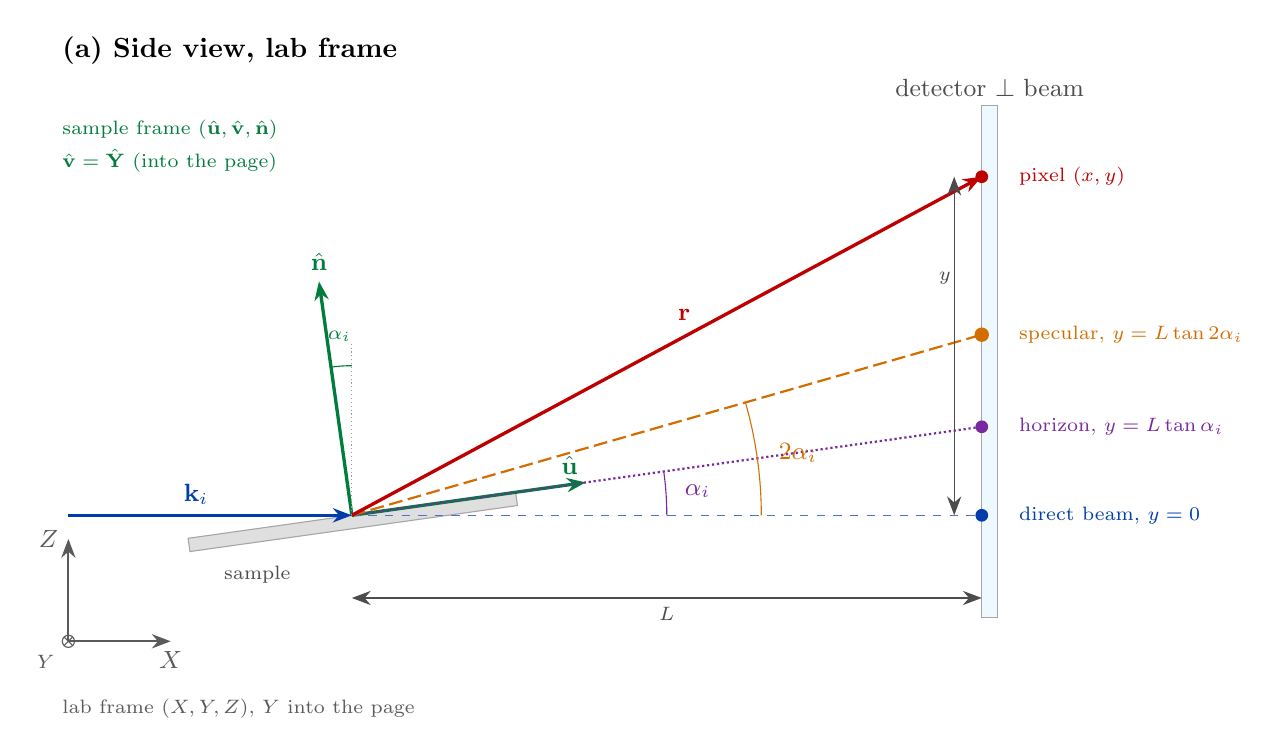
\begin{tikzpicture}[baseline=(O)]
  \pgfmathsetmacro{\yh}{\LD*tan(\AI)}
  \pgfmathsetmacro{\ys}{\LD*tan(2*\AI)}
  \pgfmathsetmacro{\aa}{\LD*cos(\AI)+\YP*sin(\AI)}
  \pgfmathsetmacro{\cc}{\YP*cos(\AI)-\LD*sin(\AI)}
  \coordinate (O) at (0,0);
  \coordinate (DB) at (\LD,0); \coordinate (H) at (\LD,\yh);
  \coordinate (S) at (\LD,\ys); \coordinate (P) at (\LD,\YP);
  \coordinate (Fa) at ({\aa*cos(\AI)},{\aa*sin(\AI)});
  \coordinate (Fc) at ({-\cc*sin(\AI)},{\cc*cos(\AI)});
  \node[font=\bfseries,anchor=west] at (-3.8,5.9) {(a) Side view, lab frame};
  % detector
  \fill[cyan!7,draw=gray!70] (\LD,-1.3) rectangle (\LD+0.2,5.2);
  \node[gray!60!black,anchor=south] at (\LD+0.1,5.2) {detector $\perp$ beam};
  % lab axes
  \draw[->,lab,thick] (-3.6,-1.6)--++(1.3,0) node[below]{$X$};
  \draw[->,lab,thick] (-3.6,-1.6)--++(0,1.3) node[left]{$Z$};
  \draw[lab] (-3.6,-1.6) circle (2.2pt); \draw[lab] (-3.6-0.055,-1.6-0.055)--(-3.6+0.055,-1.6+0.055) (-3.6-0.055,-1.6+0.055)--(-3.6+0.055,-1.6-0.055);
  \node[lab,anchor=north east,font=\scriptsize] at (-3.65,-1.65) {$Y$};
  \node[lab,anchor=west,font=\scriptsize] at (-3.8,-2.45) {lab frame $(X,Y,Z)$, $Y$ into the page};
  % tilted sample
  \begin{scope}[rotate=\AI]
    \fill[gray!25,draw=gray!70] (-2.1,-0.17) rectangle (2.1,0);
  \end{scope}
  \node[gray!60!black,font=\scriptsize] at (-1.2,-0.75) {sample};
  % sample axes
  \draw[->,sam,very thick] (O)--({3.0*cos(\AI)},{3.0*sin(\AI)}) node[above left=-1pt,sam]{$\hat{\mathbf u}$};
  \draw[->,sam,very thick] (O)--({-3.0*sin(\AI)},{3.0*cos(\AI)}) node[above,sam]{$\hat{\mathbf n}$};
  \node[sam,anchor=west,font=\scriptsize] at (-3.8,4.9) {sample frame $(\hat{\mathbf u},\hat{\mathbf v},\hat{\mathbf n})$};
  \node[sam,anchor=west,font=\scriptsize] at (-3.8,4.5) {$\hat{\mathbf v}=\hat{\mathbf Y}$ (into the page)};
  % incident beam, direct beam
  \draw[->,very thick,inc] (-3.6,0)--(O) node[pos=0.45,above,inc]{$\mathbf k_i$};
  \draw[dashed,inc!70] (O)--(DB);
  % horizon ray, specular ray
  \draw[densely dotted,hor,thick] (O)--(H);
  \draw[spc,thick,dash pattern=on 5pt off 2pt] (O)--(S);
  % pixel ray and projections
  \draw[->,very thick,sca] (O)--(P) node[pos=0.55,above left=-1pt,sca]{$\mathbf r$};
  % angles
  \pic[draw,hor,angle radius=4.0cm,"$\alpha_i$",angle eccentricity=1.1] {angle=DB--O--H};
  \pic[draw,spc,angle radius=5.2cm,"$2\alpha_i$",angle eccentricity=1.1] {angle=DB--O--S};
  \coordinate (Zt) at (0,2); \coordinate (Nt) at ({-2*sin(\AI)},{2*cos(\AI)});
  \pic[draw,sam,angle radius=1.9cm,"\scriptsize$\alpha_i$",angle eccentricity=1.2] {angle=Zt--O--Nt};
  \draw[lab!60,densely dotted] (O)--(0,2.2);
  % spots on detector
  \fill[inc] (DB) circle (2.3pt); \fill[hor] (H) circle (2.3pt);
  \fill[spc] (S) circle (2.6pt); \fill[sca] (P) circle (2.3pt);
  \node[inc,anchor=west,font=\scriptsize] at (\LD+0.35,0) {direct beam, $y=0$};
  \node[hor,anchor=west,font=\scriptsize] at (\LD+0.35,\yh) {horizon, $y=L\tan\alpha_i$};
  \node[spc,anchor=west,font=\scriptsize] at (\LD+0.35,\ys) {specular, $y=L\tan2\alpha_i$};
  \node[sca,anchor=west,font=\scriptsize] at (\LD+0.35,\YP) {pixel $(x,y)$};
  % dimensions
  \draw[<->,black!70] (0,-1.05)--node[below,font=\scriptsize]{$L$} (\LD,-1.05);
  \draw[<->,black!70] (\LD-0.35,0)--node[left,font=\scriptsize,fill=white,inner sep=1pt,pos=0.7]{$y$} (\LD-0.35,\YP);
\end{tikzpicture}
&
%====================== (b) DETECTOR FACE ======================
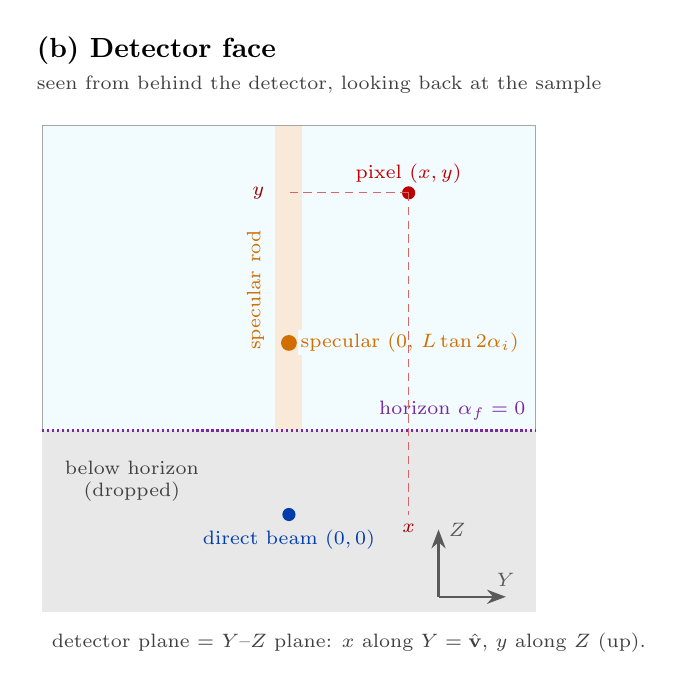
\begin{tikzpicture}[baseline=(O),scale=0.95]
  \pgfmathsetmacro{\yh}{\LD*tan(\AI)}
  \pgfmathsetmacro{\ys}{\LD*tan(2*\AI)}
  \coordinate (O) at (0,0);
  \node[font=\bfseries,anchor=west] at (-3.5,6.2) {(b) Detector face};
  \node[anchor=west,font=\scriptsize,gray!50!black] at (-3.5,5.75) {seen from behind the detector, looking back at the sample};
  \fill[cyan!5,draw=gray!70] (-3.3,-1.3) rectangle (3.3,5.2);
  % below horizon region
  \fill[gray!18] (-3.3,-1.3) rectangle (3.3,\yh);
  \node[gray!50!black,font=\scriptsize,align=center] at (-2.1,0.45) {below horizon\\(dropped)};
  % rod
  \fill[spc!15] (-0.18,\yh) rectangle (0.18,5.2);
  \node[spc,font=\scriptsize,rotate=90,anchor=south] at (-0.2,3.0) {specular rod};
  % horizon line
  \draw[hor,thick,densely dotted] (-3.3,\yh)--(3.3,\yh) node[above left,font=\scriptsize,hor]{horizon $\alpha_f=0$};
  % axes x,y
  \draw[->,lab,thick] (2.0,-1.1)--++(0.9,0) node[above,font=\scriptsize]{$Y$};
  \draw[->,lab,thick] (2.0,-1.1)--++(0,0.9) node[right,font=\scriptsize]{$Z$};
  % spots
  \fill[inc] (O) circle (2.5pt) node[below=2pt,inc,font=\scriptsize]{direct beam $(0,0)$};
  \fill[spc] (0,\ys) circle (3pt) node[right=3pt,spc,font=\scriptsize,fill=cyan!5,inner sep=1pt]{specular $(0,\,L\tan2\alpha_i)$};
  \fill[sca] (\XP,\YP) circle (2.5pt) node[above,sca,font=\scriptsize]{pixel $(x,y)$};
  \draw[sca!60,densely dashed] (\XP,\YP)--(\XP,0) (\XP,\YP)--(0,\YP);
  \node[sca!80!black,font=\scriptsize,below] at (\XP,0) {$x$};
  \node[sca!80!black,font=\scriptsize,left] at (-0.2,\YP) {$y$};
  \node[font=\scriptsize,gray!50!black,align=left,anchor=north west] at (-3.3,-1.45)
     {detector plane $=$ $Y$--$Z$ plane: $x$ along $Y=\hat{\mathbf v}$, $y$ along $Z$ (up).};
\end{tikzpicture}
\\[6mm]
%====================== (c) TOP VIEW ======================
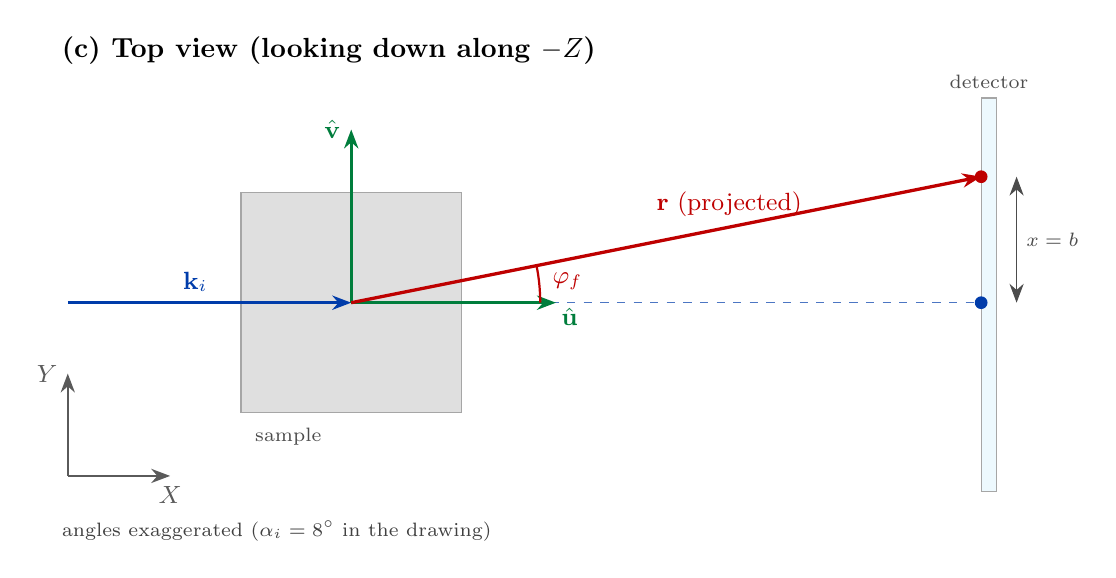
\begin{tikzpicture}[baseline=(O)]
  \coordinate (O) at (0,0);
  \coordinate (P) at (\LD,-\XP);  % Y = x ; XP negative -> draw pixel at +1.6? use |XP|
  \node[font=\bfseries,anchor=west] at (-3.8,3.2) {(c) Top view (looking down along $-Z$)};
  \fill[gray!25,draw=gray!70] (-1.4,-1.4) rectangle (1.4,1.4);
  \node[gray!60!black,font=\scriptsize] at (-0.8,-1.7) {sample};
  \fill[cyan!7,draw=gray!70] (\LD,-2.4) rectangle (\LD+0.2,2.6);
  \node[gray!60!black,anchor=south,font=\scriptsize] at (\LD+0.1,2.6) {detector};
  \draw[->,very thick,inc] (-3.6,0)--(O) node[pos=0.45,above,inc]{$\mathbf k_i$};
  \draw[dashed,inc!70] (O)--(\LD,0); \fill[inc] (\LD,0) circle (2.3pt);
  \draw[->,lab,thick] (-3.6,-2.2)--++(1.3,0) node[below]{$X$};
  \draw[->,lab,thick] (-3.6,-2.2)--++(0,1.3) node[left]{$Y$};
  \draw[->,sam,very thick] (O)--(2.6,0) node[below right=-2pt,sam]{$\hat{\mathbf u}$};
  \draw[->,sam,very thick] (O)--(0,2.2) node[left,sam]{$\hat{\mathbf v}$};
  \coordinate (Pp) at (\LD,\XP);
  \draw[->,very thick,sca] (O)--(Pp) node[pos=0.6,above,sca]{$\mathbf r$ (projected)};
  \fill[sca] (Pp) circle (2.3pt);
  \draw[<->,black!70] (\LD+0.45,0)--node[right,font=\scriptsize]{$x=b$} (\LD+0.45,\XP);
  \coordinate (Xr) at (4,0);
  \pic[draw,sca,thick,angle radius=2.4cm,"$\varphi_f$",angle eccentricity=1.15] {angle=Xr--O--Pp};
  \node[font=\scriptsize,gray!50!black,anchor=west] at (-3.8,-2.9) {angles exaggerated ($\alpha_i=8^\circ$ in the drawing)};
\end{tikzpicture}
&
%====================== (d) EQUATIONS ======================
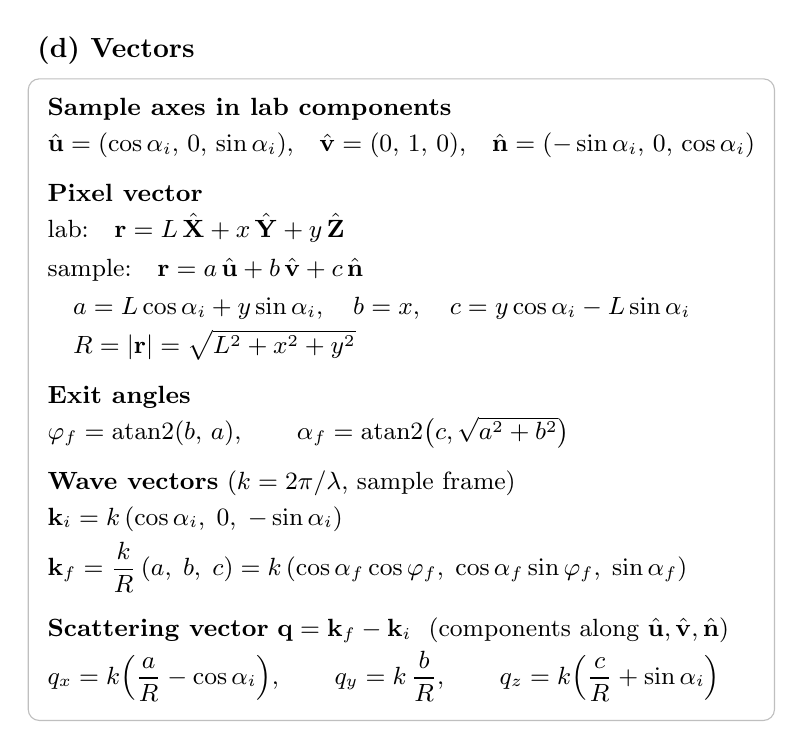
\begin{tikzpicture}[baseline=(O)]
  \coordinate (O) at (0,0);
  \node[font=\bfseries,anchor=west] at (-0.2,3.35) {(d) Vectors};
  \node[anchor=north west,align=left,draw=gray!50,rounded corners,inner sep=7pt,fill=white] at (-0.2,3.0) {%
  \textbf{Sample axes in lab components}\\[2pt]
  $\hat{\mathbf u}=(\cos\alpha_i,\,0,\,\sin\alpha_i)$,\quad
  $\hat{\mathbf v}=(0,\,1,\,0)$,\quad
  $\hat{\mathbf n}=(-\sin\alpha_i,\,0,\,\cos\alpha_i)$\\[7pt]
  \textbf{Pixel vector}\\[2pt]
  lab:\quad $\mathbf r=L\,\hat{\mathbf X}+x\,\hat{\mathbf Y}+y\,\hat{\mathbf Z}$\\[3pt]
  sample:\quad $\mathbf r=a\,\hat{\mathbf u}+b\,\hat{\mathbf v}+c\,\hat{\mathbf n}$\\[3pt]
  \quad $a=L\cos\alpha_i+y\sin\alpha_i,\quad b=x,\quad c=y\cos\alpha_i-L\sin\alpha_i$\\[3pt]
  \quad $R=|\mathbf r|=\sqrt{L^2+x^2+y^2}$\\[7pt]
  \textbf{Exit angles}\\[2pt]
  $\varphi_f=\operatorname{atan2}(b,\,a),\qquad \alpha_f=\operatorname{atan2}\!\big(c,\sqrt{a^2+b^2}\big)$\\[7pt]
  \textbf{Wave vectors} ($k=2\pi/\lambda$, sample frame)\\[2pt]
  $\mathbf k_i=k\,(\cos\alpha_i,\;0,\;-\sin\alpha_i)$\\[3pt]
  $\mathbf k_f=\dfrac{k}{R}\,(a,\;b,\;c)=k\,(\cos\alpha_f\cos\varphi_f,\;\cos\alpha_f\sin\varphi_f,\;\sin\alpha_f)$\\[8pt]
  \textbf{Scattering vector} $\mathbf q=\mathbf k_f-\mathbf k_i$ \ (components along $\hat{\mathbf u},\hat{\mathbf v},\hat{\mathbf n}$)\\[2pt]
  $q_x=k\Big(\dfrac{a}{R}-\cos\alpha_i\Big),\qquad
   q_y=k\,\dfrac{b}{R},\qquad
   q_z=k\Big(\dfrac{c}{R}+\sin\alpha_i\Big)$};
\end{tikzpicture}
\end{tabular}
\end{document}
